\chapter{\hspace*{3pt} Methods}
\label{chapter:methodology}

Automatic text classification consists of automatically assigning a predefined label to textual documents. The use of text classification can be observed in (i) organization through routing, filtering and metadata assignments; (ii) analysis, through the statistics of the labels assigned to the documents or through descriptive and predictive analyzes; and (iii) knowledge extraction, through a set of rules or values that summarize the patterns present in the collection of documents. 
Moreover, information retrieval engines which correspond to many of the use of the Internet for locating information and gaining knowledge, make use of text classification algorithms to rank the most relevant documents according to a user's query ~\cite{Manning:2008}.

To perform automatic text classification, expert systems or machine learning algorithms may be used. In the first case, one or more domain experts create a set conditional rules based on the presence or frequency of a set of words or sentences that define the class of a document. However, manually generated rules are complicated to create or update for different applications or domains and are dependent on the presence and effort of domain experts or knowledge engineers~\cite{Manning:2008}. 

For that reason, automatic text classification is one of the most studied and used areas to accomplish the tasks mentioned above. 

This chapter presents in detail the steps of our approach for the extraction and representation of document features based on the Wikipedia category graph. The implementation details for filtering and building the graph are also presented. Finally, we perform a graph-theoretic analysis of the \gls{wcg} to describe the topology of the graph and to evaluate whether graph-based techniques for semantic analysis and information retrieval can be applied to it.


\section{\hspace*{3pt} Approach} \label{sec:approach}

The rich structure of the Wikipedia Category Graph has contributed to make it a large and meaningful semantic taxonomies. That said, our main goal is to take advantage of this body of knowledge to automatically categorize any text-based content on the Web following the collective knowledge of Wikipedia contributors. A processing chain to generate a generic categorization was developed based on three steps: 

\begin{enumerate}
\item Text annotation;
\item Categories extraction; and
\item Document Representation.

\end{enumerate}
As the basis for our approach, we consider the relationships of Wikipedia Categories as a directed graph. Let $G$=($V$, $E$) be a graph, where $V$ is the set of nodes representing Wikipedia categories, and $E$ is the set of edges representing the relationships between two categories.

To make it simple to understand, let us illustrate the steps.

\subsection{\hspace*{3pt} Text Annotation} 
\label{sec:text-annotation}
When dealing with the Web of Documents, we are primarily working with unstructured data, which, in turn, hinders data manipulation and the identification of atomic elements in texts. To alleviate this problem, \gls{ie} methods, such as \gls{ner} are employed. These methods automatically extract structured information from unstructured data and make it possible to link them to external knowledge bases. 

In the context of this thesis, we chose DBpedia as our Knowledge Base because it covers many domains (Science, Arts, Politics, History, Geography, Health and Nature, among others). Another reason is its constant evolution. Since the knowledge in DBPedia is extracted from Wikipedia,  the Knowledge Base is also continuously updated by the contributors. DBpedia is also available in different languages and can be accessed either by an endpoint\footnote{\url{http://dbpedia.org/sparql/}} or being installed in a local machine, making it faster to process a vast amount of data.

Based on a comparison made by Gangemi\cite{gangemi2013comparison} we decided to used  DBpedia Spotlight tool\footnote{\url{http://dbpedia-spotlight.github.io/demo/}} for entity extraction and linking to DBpedia. Even though there are some options (such as AIDA\footnote{\url{https://github.com/codepie/aida}} or Alchemy\footnote{\url{https://www.ibm.com/watson/alchemy-api.html}}) that outperform Spotlight for the task of \gls{ner}, they fail to meet some criteria. For instance, AIDA is directly linked to YAGO and Alchemy is a paid API with limited access.  


DBpedia Spotlight is a system for automatically annotating text documents with DBpedia URIs. It contains Wikipedia's encyclopedic knowledge of about 3.5 million resources, where nearly half of the knowledge base is classified according to the following ontologies: people, organizations or places\cite{Mendes:2011}. 

The DBpedia Spotlight was used to extract and enrich entities found in the Web resources.

For instance, after processing the following Web resource using an \gls{ie} tool: ``I agree with Barack Obama that the whole episode should be investigated.", the entity  ``Barack Obama" is annotated, classified as ``person" and linked to the DBpedia resource: \\ 
 <http://dbpedia.org/resource/Barack\_Obama>, where structured information about the entity is available, as exemplified in figure \ref{fig:dbpedia-annotation}.
 
 
\begin{figure}[H]
  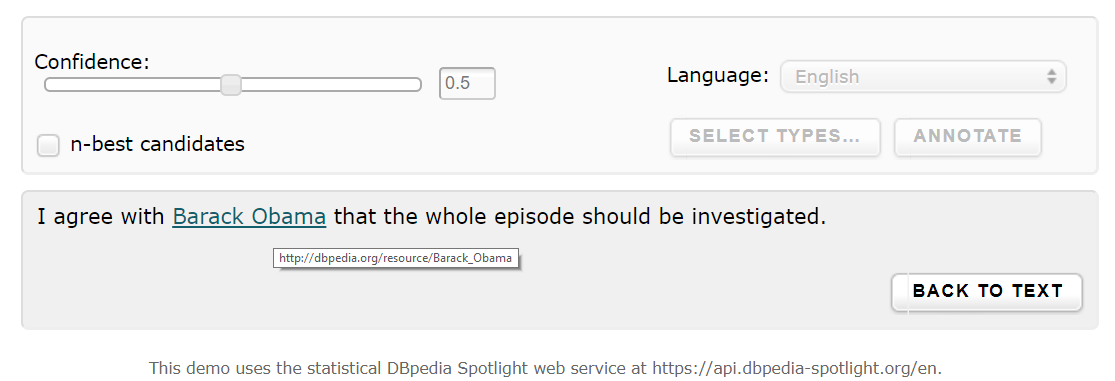
\includegraphics[width=\linewidth]{dbpedia_annotation}
  \caption{Example of text annotation by Named Entity Recognition using DBpedia SPotlight}
  \label{fig:dbpedia-annotation}
\end{figure}


 
Note that this method is language-independent as long as we have a repository of entities (such as DBpedia) and a proper annotation tool (such as DBpedia Spotlight, Apache Stanbol\footnote{\url{https://stanbol.apache.org}} or AIDA). However, the set of entities that can be identified by the annotation process is limited to the number of known entities in the dataset; in this case, DBpedia datasets in English, Dutch, French, German, Italian, Portuguese, Russian, Spanish, Hungarian and Turkish.

\subsection{\hspace*{3pt}  Categories Extraction}
\label{sec:categories-extraction}
Given the entities found in the previous step as a starting point, the categories extraction step begins by traversing the entity relationships to find a more general representation of the entity, i.e., their categories. All categories associated to the entities identified in the source of information are extracted. 

For instance, for each extracted and enriched entity in a Web resource, we explore the relationships through the predicate [dcterms:subject], which by definition represents the categories of an entity. In that sense, to retrieve the topics, we use SPARQL query language for \gls{rdf} over the DBpedia SPARQL, where we navigate up in the DBpedia hierarchy to retrieve broader semantic relations between the entities and its topics. 

Note that an entity/concept can be found in different levels of the hierarchical categories of DBpedia. Hence this approach would lead us to retrieve topics in different category levels. 

\subsection{\hspace*{3pt} Representation of Document}
\label{sec:doc-representation}

The goal of this step is to figure out how the resource page being tagged is related to a more generic subset of Wikipedia categories. 

In the top of Wikipedia categorization stricture, under the ``Contents" category there is the category ``Main topic classifications"\footnote{\url{https://en.wikipedia.org/wiki/Category:Main_topic_classifications}} that has 19 subcategories representing different fields of study, hence we used the subcategories of ``Main topic classifications" as a subset of the Wikipedia Categories for the context of this thesis. 

The algorithm \ref{alg:fingerprint-generation} begins with the categories assigned to entities recognized in the text and generates a categorization based on the frequency of assignments with the top-level categories in Wikipedia, the so-called Main topic classifications.

To define the problem of automatically assigning categories to resources let $D = \{d_1,d_2,d_3,\ldots\,d_n\}$ be a finite set of documents and $C = \{c_1,c_2,c_3,\ldots\,c_n\}$ a finite set of predefined categories.
The problem is finding a function $f: D \times C \mapsto \mathbb{R}$ that assigns a score $s$ for each pair 
$\{d_i, c_i\} \in  D \times C $. The document $d_i$ is assigned to a class $c_i$ if $s$ is greater than predefined threshold, $\{d_i, c_i\} > \tau$. 


Our approach consists of navigating in the Category Graph from each category extracted in the previous step towards the top of the graph by all the shortest paths between the category and the main topics.  

The Category Graph is not a perfect hierarchical structure. It is noisy, contains cycles and many of the paths from a category to the main topic classifications do not make sense. One of the main reasons for that is that users who add categories to Wikipedia pages often assign them to small grained categories in the graph. Most of the time they don't fully understand the internal structure of the graph and don't fallow the guidelines when choosing particular categories. The category graph as well as the content of the articles can be changed over time, also changing the original intent of the author and the meaning of the category assignments.

Since the Category Graph is being used as a taxonomy, we decided to use the shortest path to alleviate this problem. We based our decision on the results of previous works. Kittur\cite{knuth:84} tested many heuristics and the shortest paths between categories showed to be the best approach. 

Strube and Ponzetto\cite{strube2006wikirelate} developed a system named WikiRelate!. They used data from Wordnet, Wikipedia, and Google for computing degrees of semantic similarity and reported that Wikipedia outperforms Wordnet.  They used different measures for computing semantic relatedness and showed good results with the one based on shortest paths.

Each time the source category reaches one of the top-level categories by the shortest paths, we update the influence of this top category in the composition of the resource classification.

Based on the influence of each main topic category in the resource being tagged, we generate a representation of the document based on the calculated categorization as a multidimensional vector.

The \gls{vsm} is a simple, traditional and practical model that makes it possible to represent documents as vectors and perform any algebraic operation to compare them ~\cite{salton1988term}.

In this method, the documents of a collection $D$ are represented in the VSM as points in a multidimensional Euclidean space, where each dimension corresponds to a distinct term in that collection. The set $T$ of distinct terms of collection $D$, called vocabulary collection of $D$, is obtained in a process called lexical analysis.

Each term of the set $T$ can be composed of only one word (unigrams), several words (bigrams, trigrams or n-grams) or sentences, and has an associated weight to determine its degree of importance ~\cite{salton1988term}.

Given a document $d_i \in D$, this document is formally represented in the VSM as follows:

$d={w_{i1},w_{i2},w_{i3},\ldots,w_{i|T|}}$,

where $T$ is the vocabulary set of the collection $D$ and $w_{ij} (1 \le j \le |T|)$ is the weight of the term $t_j$ in the document $d_i$, such that $w_{ij} = 0$ if the term $t_j$ does not occur in the document $d_i$.

As a formal definition of our approach, lets denote $I$ as the set of categories related to a web resource $d$, found in the category extraction step. $C$ is the set of all Categories in Wikipedia and $M$ is the set of categories that represent the main topics. $G = (V,E)$, where $I \subset V ; C \subset V ; M \subset V$; and $M \subset C$.  The parameter  $l$ is defined to indicate the broadest $l$ levels to be considered in the set of $M$. If $t$ is 1, only the main topics previously defined are considered; if $t$ is 2, any category 1 edge away in the graph is also considered as a main topic. The weight $w$ is defined to make it possible to assign different weights for 

Note that a path is a sequence of graph vertices visited from a given category $c \in C$ to a main topic $m \in M$.  

\begin{algorithm}
\caption{Vector Generation}\label{alg:fingerprint}
\label{alg:fingerprint-generation}
\begin{algorithmic}[1]
\Procedure{GenerateVector}{$G,M, I, t, w$}
\State $E\gets$ a map from a list of categories $ m \in M$
\For {$i \in I$}
\State $S\gets$ the set of shortest paths between $i$ and any category in $M$
\For {$s \in S$}
\State $B\gets$ the set of last $t$ vertices in path $s$
\For {$b \in B$}
\State $E[b]\gets E[b] + w$
\EndFor
\EndFor
\EndFor
\State \textbf{return} $E$
\EndProcedure
\end{algorithmic}
\end{algorithm}


In all experiments described in this paper, only the subcategories of Main\_top\_classifications were considered in the set of  $M$ (i.e. Arts, Culture,Games,Geography,Health, History, Humanities, Industry, Law, Life, Mathematics, Matter, Nature, Philosophy, People, Reference works, Religion, Science and technology and Society) it means that we fixed the parameter $t$ with a value of $1$. In effect, as a result of this method we have a 19-sized vector, representing the content of a given text-based resource.

\section{\hspace*{3pt} A running example}

To illustrate how the method works in a real application scenario, we present a step-by-step example in a text extracted from the Internet.

The text is an excerpt from the article entitled ``Market Totalitarianism in North Korea", taken from The New York Times\footnote{\url{https://www.nytimes.com/}} of May 3, 2017: \

\textit{"(...) Post-Communist, postindustrial, kleptocratic dynastic regime of North Korea may become the crown jewel of the new axis-of-tyranny ideology (...)"}\footnote{\url{https://nyti.ms/2py3z4r}} \

\subsection{\hspace*{3pt} Processing step 1 - Text Annotation} 

As mentioned in section \ref{sec:text-annotation}, our approach starts by extracting structured data from unstructured text by recognizing the named entities present in the text-based resource and linking them to DBpedia. 

After using DBpedia Spotlight to extract the concept from the excert, we obtain the entities linked to DBpedia as shown in table \ref{tab:example-entities}.

% Please add the following required packages to your document preamble:
% \usepackage{booktabs}
\begin{table}[H]
\centering
\caption{Entities extracted from the text and their respective links to DBpedia concepts.}
\label{tab:example-entities}
\begin{tabular}{@{}ll@{}}
\toprule
Entity in Text & Link to Dbpedia                                  \\ \midrule
postindustrial & http://dbpedia.org/resource/Post-industrial\_society \\
kleptocratic   & http://dbpedia.org/resource/Kleptocracy              \\
dynastic       & http://dbpedia.org/resource/Dynasty                  \\
North Korea    & http://dbpedia.org/resource/North\_Korea             \\
tyranny        & http://dbpedia.org/resource/Tyrant                   \\ \bottomrule
\end{tabular}
\end{table}


\subsection{\hspace*{3pt} Processing step 2 - Categories Extraction}

As described in the section \ref {sec:categories-extraction}, the second step consists of extracting all categories related to all entities found in the text.
Using a \gls{sparql} query that retrieves all categories (dc:subject predicate) associated with the entities listed in table \ref{tab:categorylinks} we obtain the categories listed in table \ref{tab:entities-categories}.


\begin{table}[H]
\centering
\caption{List of all entities extracted from the example test and the categories associated to them}
\label{tab:entities-categories}
\begin{tabular}{@{}ll@{}}
\toprule
\textbf{Entity}         & \textbf{Categories}                                                                                                                                                                                                                                                                                                                                                                                                        \\ \midrule
Post-industrial society & \begin{tabular}[c]{@{}l@{}}Postindustrial society \\ Information economics\\ Postmodernism\\ Social philosophy\\ Technology in society\\ Theories of history\end{tabular}                                                                                                                                                                                                                                                  \\
\rowcolor[HTML]{EFEFEF} 
Kleptocracy             & \begin{tabular}[c]{@{}l@{}}Forms of government\\ Political corruption\\ Political terminology\end{tabular}                                                                                                                                                                                                                                                                                                                 \\
Dynasty                 & \begin{tabular}[c]{@{}l@{}}Royal families\\ History-related lists\\ Monarchy\end{tabular}                                                                                                                                                                                                                                                                                                                                  \\
\rowcolor[HTML]{EFEFEF} 
North Korea             & \begin{tabular}[c]{@{}l@{}}1948 establishments in North Korea\\ Communist states\\ Countries in Asia\\ East Asian countries\\ Korea\\ Korean-speaking countries and territories\\ Member states of the United Nations\\ Military dictatorships\\ North Korea\\ Northeast Asian countries\\ One-party states\\ Republics\\ Socialist states\\ States and territories established in 1948\\ Totalitarian states\end{tabular} \\
tyranny                 & \begin{tabular}[c]{@{}l@{}}Ancient Greek government\\ Ancient Greek titles\\ Ancient Roman government\\ Positions of authority\\ Ancient Greek tyrants\end{tabular}                                                                                                                                                                                                                                                        \\ \bottomrule
\end{tabular}
\end{table}


\subsection{\hspace*{3pt} Processing step 3 - Document Representation}

In this last step, as detailed in section \ref{sec:doc-representation}, we generate a vector that represents the document based on the count of shortest paths between all categories associated with entities extracted from the text-based resource and a set of more generic categories in the \gls{wcg}. The induced graph for this example contains 143 distinct categories and 256 relationships and can be seen in figure \ref{fig:graph-example}.

 
\begin{figure}[H]
  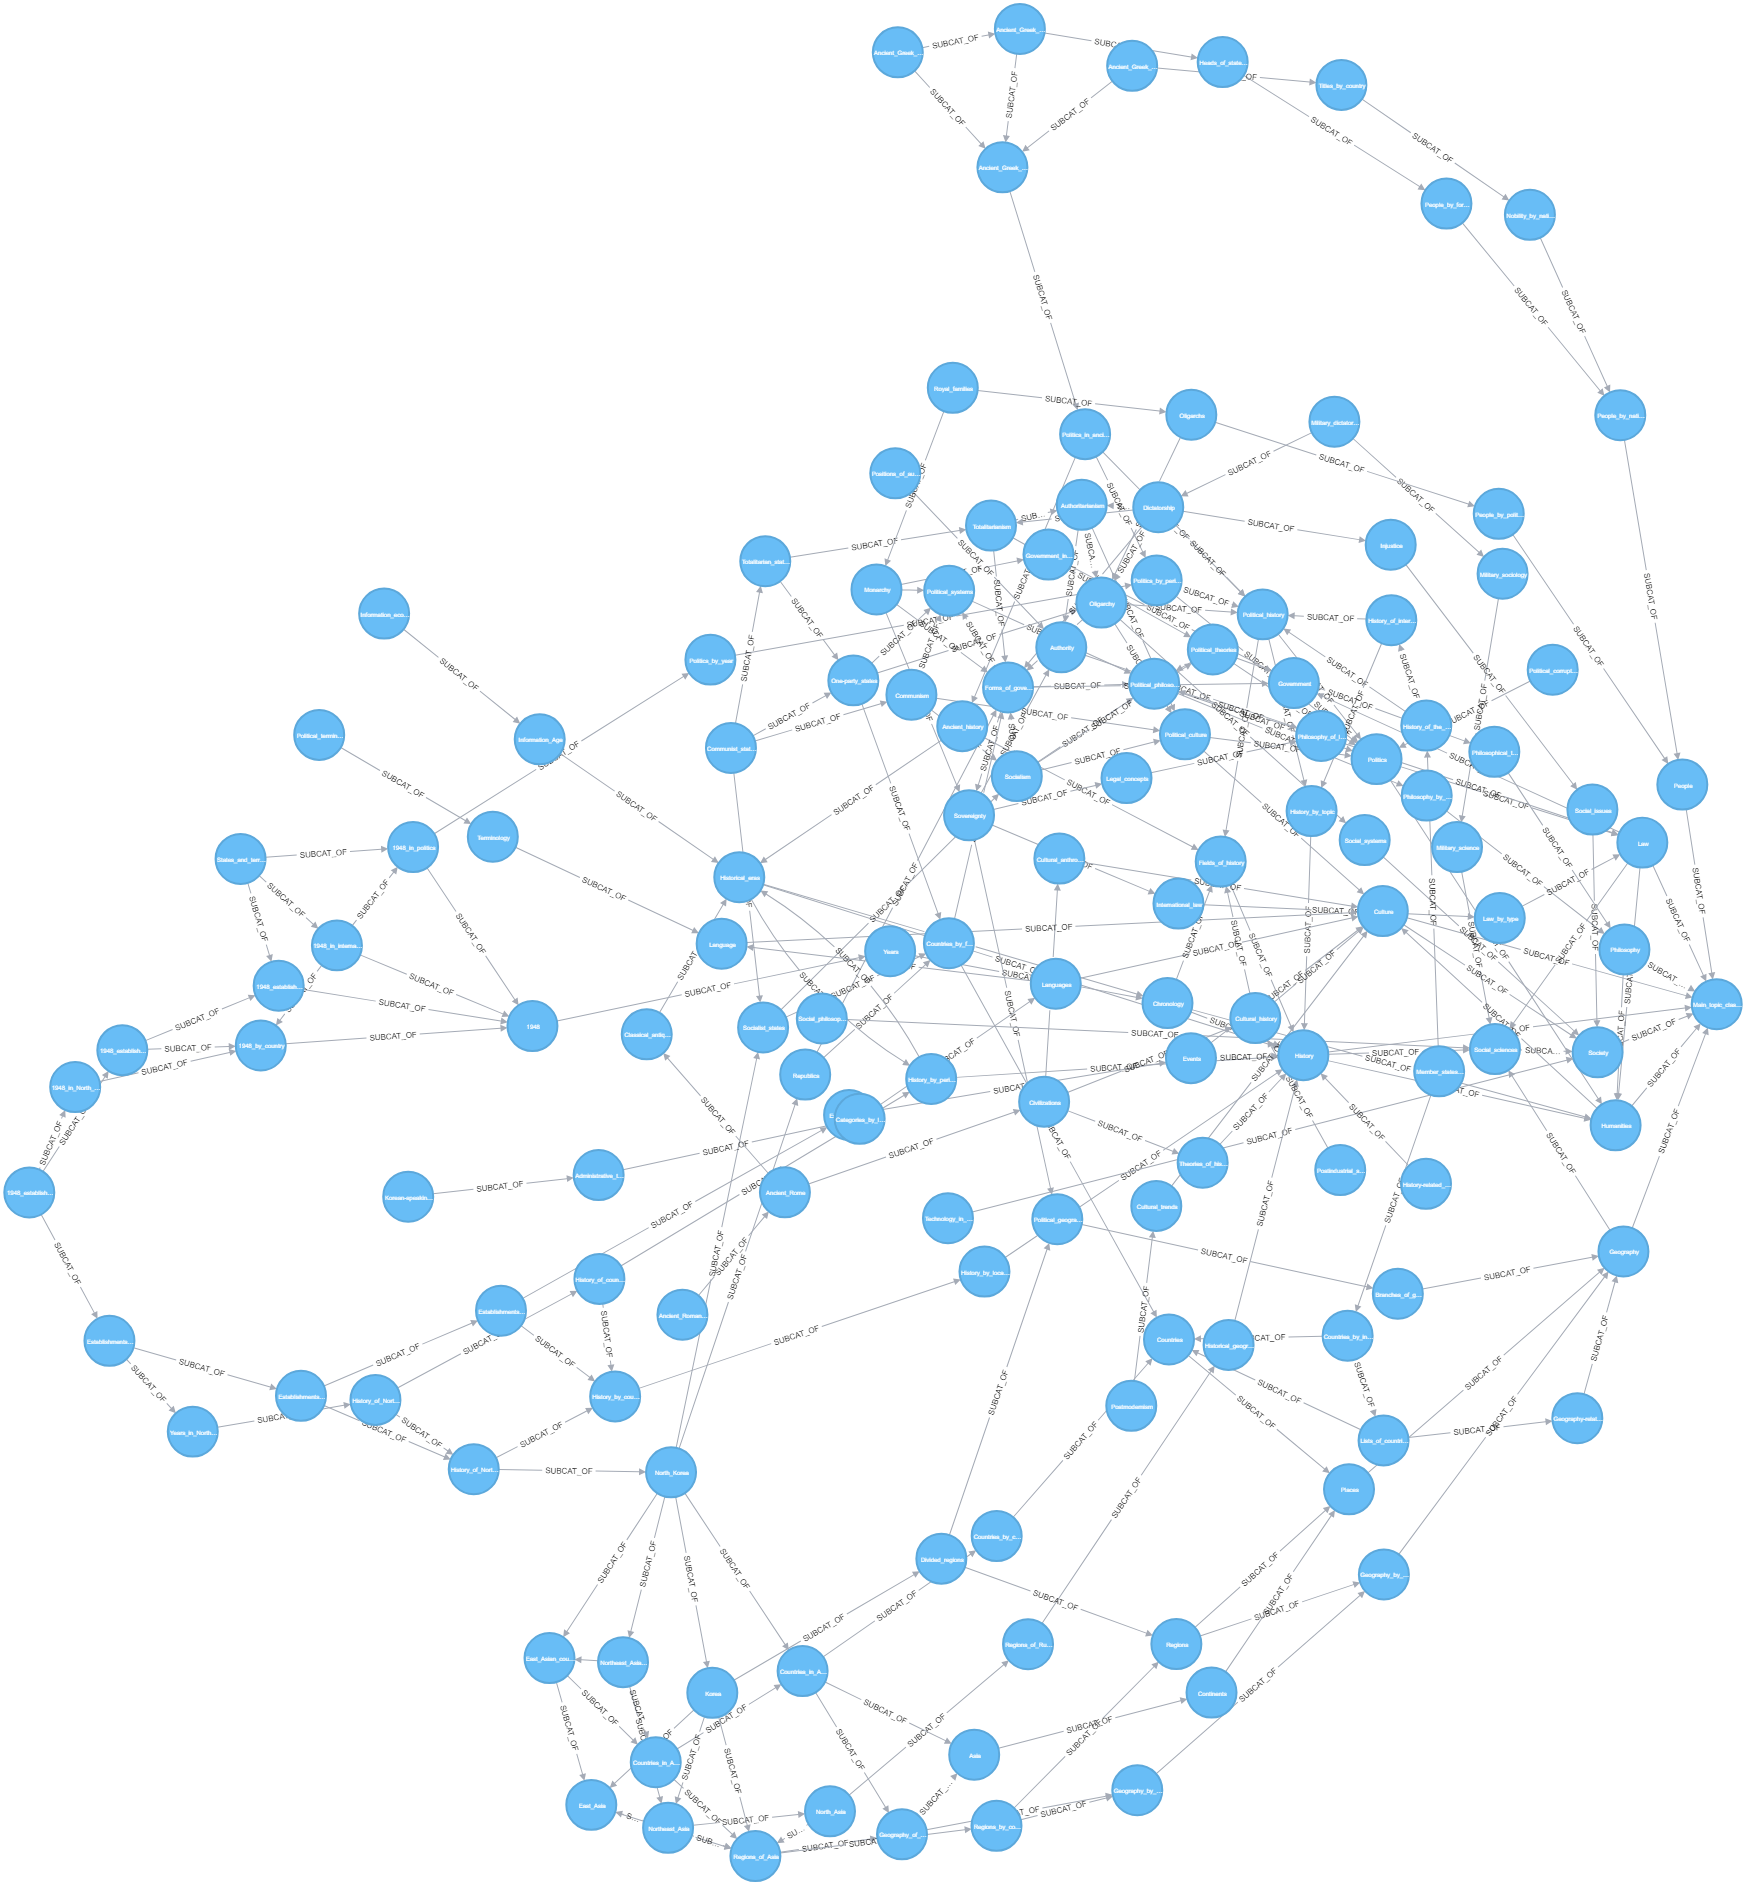
\includegraphics[width=\linewidth]{graph-example}
  \caption{Induced graph containing all shortest paths from the categories found and described in table in \ref{tab:entities-categories} and ``Main topic classifications" (on the right of the graph)}
  \label{fig:graph-example}
\end{figure}


The vector generated for this examples is shown in table \ref{tab:vector}. Note that this is the representation of the document based only on a small excerpt. 
We can infer that this document is strongly related to History, Humanities, Law, and Culture, and also has some weaker relatedness to Society, Geography, Philosophy, and People. Bellow we present one random example of path for each top-level category that contributed for the document representation.


\begin{itemize}

\item Theories of history $\rightarrow$ \textbf{History} 

\item Political corruption $\rightarrow$ Politics $\rightarrow$ \textbf{Humanities}

\item Political corruption $\rightarrow$ Politics $\rightarrow$ \textbf{Law} 


\item Totalitarian states $\rightarrow$ Totalitarianism $\rightarrow$ Authoritarianism $\rightarrow$ Political culture $\rightarrow$ \textbf{Culture}


\item Military dictatorships $\rightarrow$ Dictatorship $\rightarrow$ Oligarchy $\rightarrow$ Social systems $\rightarrow$ \textbf{Society} 


\item 
Korea $\rightarrow$ Divided regions $\rightarrow$ Political geography $\rightarrow$ Branches of geography $\rightarrow$ \textbf{Geography}


\item Forms of government $\rightarrow$ Political philosophy $\rightarrow$ Philosophy by topic $\rightarrow$ \textbf{Philosophy}

\item Royal families $\rightarrow$ Oligarchs $\rightarrow$ People by political orientation $\rightarrow$ \textbf{People} 


\end{itemize}


% Please add the following required packages to your document preamble:
% \usepackage{booktabs}
\begin{table}[H]
\centering
\caption{19-sized vector representing the document based on the top-level categories of \gls{wcg}}
\label{tab:vector}
\begin{tabular}{@{}ll@{}}
\toprule
Top-level Categories     & Shortest paths \\ \midrule
History                  & 29             \\
Humanities               & 23             \\
Law                      & 21             \\
Culture                  & 17             \\
Society                  & 9              \\
Geography                & 8              \\
Philosophy               & 5              \\
People                   & 3              \\
Religion                 & 0              \\
Matter                   & 0              \\
Life                     & 0              \\
Industry                 & 0              \\
Games                    & 0              \\
Arts                     & 0              \\
Science\_and\_technology & 0              \\
Health                   & 0              \\
Reference\_works         & 0              \\
Nature                   & 0              \\
Mathematics              & 0              \\ \bottomrule
\end{tabular}
\end{table}






\section{\hspace*{3pt}Implementation Details}
In the scope of this thesis, finding the paths between entities and a set of top categories requires that the structure of Wikipedia Category is represented so that computer programs can navigate on it. 

Therefore, we needed a way of representing the available information about the Wikipedia structure as a graph. The Wikipedia Category Graph consists of Wikipedia pages with the “Category:” prefix such as “Category:Law”. The graph is extracted by finding links between category pages. In other words, a category page is liked to another category page that is broader in scope.

To perform this task, we obtained a dump of the files enwiki-latest-page.sql, enwiki-latest-category.sql and enwiki-latest-categorylinks.sql, of October 2016 \footnote{\url{https://dumps.wikimedia.org/enwiki/20161020\/}}.

These files consist the structure of Wikipedia represented in a MySQL relational database.

The file enwiki-latest-categorylinks.sql.gz contains the information needed to extract the categories-categories and categories-articles relations. The information is represented in the file as INSERT statements where all entries are on the form: \\
\textit{
(cl\_from,cl\_to,cl\_sortkey,cl\_timestamp,cl\_sortkey\_prefix,cl\_collation,cl\_type). }



\begin{table}[H]
\begin{adjustbox}{width=1\textwidth}
\begin{tabular}{@{}ll@{}}
\toprule
Field               & Description                                                                                                   \\ \midrule
cl\_from            & Stores the page.page\_id of the article where the link was placed                                             \\
cl\_to              & Stores the name (excluding namespace prefix) of the desired category. Spaces are replaced by underscores (\_) \\
cl\_sortkey         & Stores the title by which the page should be sorted in a category list.                                       \\
cl\_timestamp       & Stores the time at which that link was last updated in the table.                                             \\
cl\_sortkey\_prefix & either an empty string if a page is using the default sortkey or a human readable version of cl\_sortkey.     \\
cl\_collation       & What collation is in used.                                                                                    \\
cl\_type            & What type of article is this (file, subcat (subcategory) or page (normal page)).                              \\ \bottomrule
\end{tabular}
\end{adjustbox}
\caption{Description of fields in INSERT statements for the table categorylinks.}
\label{tab:categorylinks}
\end{table}

<EXAMPLE OF INSERT STATEMENTS HERE>

Considering the goal of this process is to represent the underlying Wikipedia category structure as a graph, we chose to use Neo4J \footnote {\url{https://neo4j.com/}}, a graph-based database that provides a free version and proper documentation, as well as an active community. 

Even though only the category graph is needed, it was necessary to extract the page file as well, since the identifier of the categories refers not to the categories themselves, but to the page about the categories. For this step, a parser was developed in python. First, the file containing all the pages of Wikipedia is scanned and, through a regular expression, the data is filtered.

The output is a CSV file with three fields: page identifier, page title, and namespace. Namespaces are a Wikipedia internal classification system to identify what a page refers to, such as an article, a category, user page, or other classifications. Articles are identified with namespace 0 and categories with namespace 14, for example.
The second step is to go through the file that corresponds to the categories of Wikipedia. The output of this step is a CSV file with two properties: page identifier and category title. From this file, it is possible to link the categories and the corresponding pages. The third and final step of this step is the extraction of links between categories. The data is extracted from the file of the enwiki-latest-categorylinks.sql file, and the output is a csv file with two properties: page identifier for the source category and page identifier for destination category.

Administrative categories are used for Wikipedia internal organization and mantaining. They were ignored during processing and are not in the final files. Examples of these categories include, but are not limited to, categories that begin with \textit{Articles\_needing\_} and \textit{WikiProject\_}, named hidden categories.


These categories provide a tool for grouping pages with features in common so that publishers can quickly identify where improvements are needed. Although these categories are essential for the maintenance and administration of the encyclopedia, they are not relevant to end users and were removed in the context of the work for two reasons: 1) They add complexity to the structure of the graph 2) They do not semantically describe articles associated to them and therefore do not add relevant information to the paths.


The ideal paths between a set of categories has no hidden categories. Thus, the hidden categories must be removed in such a way that the information is not lost because a hidden category can be a subcategory of a visible category or they can have visible categories as their subcategories

<EXAMPLE OF HIDDEN CATEGORIES REMOVAL HERE>

After processing the Wikipedia dump files,  it is possible to generate the complete graph of categories. First, we import all the pages referring to categories in the Neo4J, and then the relations between them are imported. The generated graph has only a $Category$ concept with the $categoryName$ and $categoryID$ properties and a $SUBCATEGORY\_OF$ relationship type, with no properties.

The example below illustrates how information retrieval works in a Neo4J graph.

The example returns all nodes of type$ Category$  that are connected to another node of type $Category$ that have the property $CategoryName$ with the value equals to Carnivores for the $SUBCATEGORY_OF$ property. In this case, all subcategories of Carnivores are retrieved.

\begin{verbatim}
MATCH (a: Category) - [r: SUBCATEGORY_OF] ->
(b: Category {categoryName: ""}) RETURN a
\end{verbatim}





